\chapter{Background e Stato dell'Arte}

L'evoluzione del panorama delle minacce informatiche ha reso indispensabile lo sviluppo di tecniche e strumenti sempre più sofisticati per l'analisi forense digitale. Questo capitolo fornisce le basi teoriche necessarie per comprendere il contesto in cui si inserisce il presente lavoro, esplorando i concetti fondamentali del Digital Forensics and Incident Response (DFIR), con particolare attenzione all'analisi della memoria volatile. Verranno inoltre esaminati i principali framework esistenti. Infine, verrà illustrato cosa è YARA e quali sono i suoi principali utilizzi nell'ambito dell'analisi forense e della rilevazione di minacce.

\section{Digital Forensics e Incident Response (DFIR)}

\subsection{Definizione e principi fondamentali}

Il Digital Forensics and Incident Response (DFIR) rappresenta la convergenza di due discipline complementari che, insieme, formano il nucleo delle capacità di risposta alle minacce cyber moderne. Il termine DFIR è stato coniato per riflettere la natura interconnessa di queste attività nel contesto operativo reale.\\

La \textbf{Digital Forensics} è definita dal NIST come "l'applicazione di scienza e metodi per identificare, preservare, raccogliere, validare, analizzare, interpretare, documentare e presentare evidenze digitali derivate da fonti digitali allo scopo di facilitare o promuovere la ricostruzione di eventi" \cite{kent2006}. Questa disciplina si basa su quattro principi scientifici fondamentali:

\begin{itemize}
    \item \textbf{Preservazione dell'evidenza}: Garantire che i dati non vengano alterati durante l'acquisizione e l'analisi
    \item \textbf{Chain of custody}: Documentare ogni passaggio per mantenere l'ammissibilità legale
    \item \textbf{Ripetibilità}: Le analisi devono produrre risultati consistenti quando ripetute
    \item \textbf{Documentazione completa}: Ogni azione deve essere registrata e giustificata
\end{itemize}

Questi principi sono ulteriormente codificati negli standard internazionali come ISO/IEC 27037:2012 \cite{iso27037}, che fornisce linee guida per l'identificazione, raccolta, acquisizione e preservazione delle evidenze digitali. Lo standard enfatizza quattro principi cardine: rilevanza, affidabilità, sufficienza e conformità alle normative locali. Similmente, le linee guida SWGDE \cite{swgde2022} per l'acquisizione di contenuti online stabiliscono best practices specifiche per la preservazione di evidenze volatili come pagine web, social media e comunicazioni cloud-based.\\

L'\textbf{Incident Response}, d'altra parte, si concentra sulla gestione operativa degli incidenti di sicurezza con l'obiettivo di minimizzare l'impatto e ripristinare le operazioni normali nel minor tempo possibile. Il SANS Institute definisce l'IR come "un approccio organizzato per affrontare e gestire le conseguenze di una violazione della sicurezza o di un attacco informatico" \cite{sans2023}.\\

La fusione di queste discipline nel DFIR riconosce che, nel mondo reale, l'analisi forense e la risposta agli incidenti sono attività inseparabili. Durante un incidente attivo, i responder devono bilanciare molteplici esigenze contrastanti: contenere la minaccia mentre preservano le evidenze, analizzare i sistemi compromessi senza interrompere le operazioni critiche, e trovare il giusto equilibrio tra la necessità di un'indagine approfondita e l'urgenza del ripristino operativo.

\subsection{Fasi del processo DFIR}

Il processo DFIR segue un approccio strutturato che può essere suddiviso in sei fasi principali, come definito dal framework NIST SP 800-61 \cite{cichonski2012}. Mentre queste fasi forniscono una struttura logica, è importante comprendere che nella pratica spesso si sovrappongono e richiedono iterazioni multiple.

\begin{figure}[ht]
    \centering
    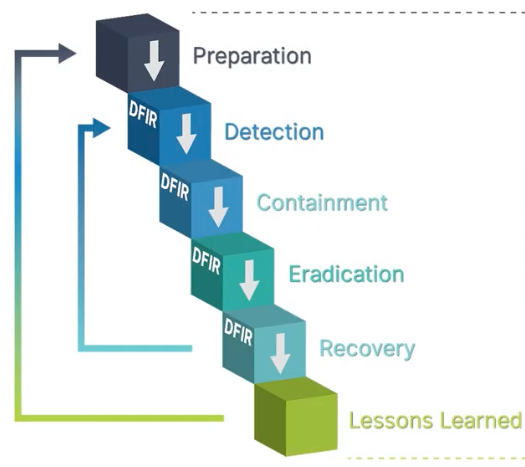
\includegraphics[width=0.6\linewidth]{images/stato-arte/digital-forensics-incident-response-plan-flow.png}
\end{figure}

\paragraph{1. Preparazione (Preparation)}
La fase più critica e paradossalmente più trascurata del processo DFIR. Un'organizzazione ben preparata può rispondere a un incidente in ore invece che in giorni. La preparazione include:
\begin{itemize}
    \item Sviluppo di playbook e procedure operative standard (SOP) per scenari comuni
    \item Configurazione di strumenti e infrastrutture di analisi prima che servano
    \item Training regolare del personale attraverso simulazioni realistiche di incidenti
    \item Implementazione di meccanismi di logging e monitoraggio pervasivi
    \item Predisposizione di capacità di acquisizione forense ready-to-use
\end{itemize}

\paragraph{2. Identificazione (Detection)}
Il rilevamento tempestivo e l'accurata identificazione di un incidente possono fare la differenza tra un minor inconveniente e una catastrofe aziendale. Questa fase richiede:
\begin{itemize}
    \item Analisi degli alert provenienti da molteplici sistemi di sicurezza
    \item Triage iniziale per distinguere falsi positivi da minacce reali
    \item Determinazione dello scope iniziale e della potenziale gravità
    \item Attivazione del team di risposta con le competenze appropriate
\end{itemize}

\paragraph{3. Contenimento (Containment)}
Una volta confermato l'incidente, il contenimento diventa prioritario per limitare i danni. Si articola in due approcci complementari:
\begin{itemize}
    \item \textit{Contenimento a breve termine}: Azioni immediate come isolare sistemi compromessi dalla rete
    \item \textit{Contenimento a lungo termine}: Misure sostenibili come applicazione di patch temporanee mentre si prepara l'eradicazione completa
    \item Backup forensi dei sistemi affetti prima di qualsiasi modifica
    \item Documentazione meticolosa di ogni azione per preservare la chain of custody
\end{itemize}

\paragraph{4. Eradicazione (Eradication)}
La rimozione completa della minaccia richiede precisione chirurgica per evitare che l'incidente si ripresenti:
\begin{itemize}
    \item Identificazione e rimozione di tutti gli artefatti malevoli, inclusi backdoor nascoste
    \item Chiusura definitiva delle vulnerabilità sfruttate dall'attaccante
    \item Rafforzamento delle difese per prevenire tecniche simili in futuro
    \item Verifica dell'assenza di persistence mechanisms lasciati dall'attaccante
\end{itemize}

\paragraph{5. Recupero (Recovery)}
Il ripristino delle operazioni normali deve essere gestito con cautela per evitare la reintroduzione della minaccia:
\begin{itemize}
    \item Ricostruzione dei sistemi da backup verificati puliti
    \item Monitoraggio intensificato per settimane per rilevare eventuali ricomparse
    \item Validazione sistematica del ripristino di tutte le funzionalità business-critical
    \item Implementazione di controlli compensativi temporanei dove necessario
\end{itemize}

\paragraph{6. Lessons Learned}
Spesso trascurata per la fretta di "chiudere" l'incidente, questa fase è cruciale per il miglioramento continuo:
\begin{itemize}
    \item Documentazione dettagliata dell'intero incidente e della risposta
    \item Identificazione onesta di cosa ha funzionato e cosa no
    \item Aggiornamento di procedure, playbook e training basato sull'esperienza
    \item Condivisione di IOC e lessons learned con la community (nei limiti della confidenzialità)
\end{itemize}

È fondamentale comprendere che l'analisi forense non è confinata a una singola fase ma permea l'intero processo, fornendo le informazioni necessarie per decisioni informate in ogni momento.

\subsection{Importanza nell'ambito della cybersecurity moderna}

Il DFIR ha assunto un ruolo centrale nella cybersecurity moderna per diverse ragioni interconnesse che riflettono l'evoluzione del panorama delle minacce e del contesto normativo. Le minacce moderne hanno raggiunto livelli di sofisticazione che richiedono capacità DFIR avanzate per essere contrastate efficacemente:

\paragraph{Advanced Persistent Threats (APT)} rappresentano attaccanti sponsorizzati da stati nazionali o crime syndicate organizzati che mantengono una presenza persistente nelle reti delle vittime per mesi o anni, muovendosi lateralmente ed estraendo dati di valore strategico con l'obiettivo di monetizzarli rivendendoli nei marketplace del dark web, ricattare le organizzazioni minacciando la divulgazione o la distruzione dei dati, oppure ottenere vantaggi geopolitici o industriali a favore dei propri mandanti.

\paragraph{Ransomware-as-a-Service (RaaS)}, come modello, ha democratizzato gli attacchi ransomware, permettendo anche a criminali con competenze tecniche limitate di lanciare attacchi devastanti. I fornitori di RaaS gestiscono l'infrastruttura, forniscono il malware e negoziano i riscatti, prendendo una percentuale dei profitti.

\paragraph{Supply chain attacks} sfruttano la fiducia intrinseca nelle relazioni commerciali, compromettendo fornitori di software o servizi per raggiungere i veri target. L'attacco SolarWinds \cite{solarwinds2020} ha dimostrato come un singolo fornitore compromesso possa impattare migliaia di organizzazioni.

\paragraph{Tecniche Living-off-the-land} utilizzano esclusivamente tool legittimi già presenti nel sistema - PowerShell, WMI, scheduled tasks - per condurre attività malevole, rendendo la detection estremamente difficile poiché non c'è malware tradizionale da rilevare.

\paragraph{Requisiti normativi e compliance}
Il panorama normativo moderno ha trasformato il DFIR da best practice a requisito legale con pesanti sanzioni per non conformità. Il GDPR \cite{gdpr2016} richiede la notifica delle violazioni entro 72 ore con documentazione dettagliata dell'incidente, delle misure prese e dell'impatto sui dati personali. La direttiva NIS2 \cite{nis2_2022} estende requisiti simili agli operatori di servizi essenziali e fornitori digitali importanti. DORA (Digital Operational Resilience Act) \cite{dora2022} stabilisce standard ancora più stringenti per il settore finanziario, richiedendo capacità di incident response testate e validate regolarmente.

\paragraph{Riduzione del tempo di permanenza (dwell time)}
Secondo il Mandiant M-Trends 2023 \cite{mandiant2023}, il tempo medio globale di permanenza degli attaccanti nelle reti è sceso a 16 giorni, ma questo nasconde una realtà bimodale: organizzazioni con capacità DFIR mature rilevano intrusioni in giorni, mentre quelle senza possono ospitare attaccanti per mesi . Ogni giorno di permanenza aumenta esponenzialmente il rischio di esfiltrazione di dati critici, movimento laterale verso sistemi più sensibili, e establishment di meccanismi di persistenza difficili da eradicare.

\paragraph{Intelligence e prevenzione}
Il DFIR moderno non è solo reattivo ma contribuisce attivamente alla postura di sicurezza proattiva dell'organizzazione. Ogni incidente gestito genera Threat Intelligence preziosa: indicatori di compromissione (IOC) che possono essere condivisi per protezione collettiva, comprensione delle Tactics, Techniques, and Procedures (TTP) degli attaccanti per migliorare le difese, identificazione di gap nelle difese da colmare con priorità, e lezioni operative che migliorano la risposta futura.

Questa intelligence, quando propriamente raccolta e analizzata, trasforma ogni incidente da crisi da gestire a opportunità di apprendimento e rafforzamento, creando un ciclo virtuoso di miglioramento continuo.

\section{Memory Forensics}

\subsection{Concetti base della memoria volatile}

La memoria volatile, principalmente la RAM (Random Access Memory), rappresenta lo stato "vivo" di un sistema informatico in un dato istante. A differenza dello storage persistente che mantiene i dati anche senza alimentazione, la memoria volatile contiene informazioni che esistono solo mentre il sistema è acceso, rendendola paradossalmente sia fragile che estremamente rivelatrice dal punto di vista forense \cite{ligh2014}.

\subsubsection{Architettura della memoria}
La memoria moderna segue una gerarchia complessa progettata per bilanciare velocità, capacità e costo:

\begin{itemize}
    \item \textbf{Registri CPU}: Storage ultra veloce (accesso in 1 ciclo clock) ma capacità minima (KB)
    \item \textbf{Cache L1/L2/L3}: Buffer progressivamente più grandi ma più lenti tra CPU e RAM
    \item \textbf{RAM principale}: Area di lavoro primaria del sistema (GB), accesso in ~100 cicli
    \item \textbf{Memory-mapped I/O}: Regioni speciali per comunicazione diretta con dispositivi hardware
\end{itemize}

Dal punto di vista forense, la RAM principale è il target primario poiché contiene la visione più completa dello stato del sistema. La sua organizzazione logica include lo \textbf{spazio kernel} con le strutture critiche del sistema operativo, driver e tabelle di sistema; lo \textbf{spazio utente} dove risiedono processi applicativi, le loro librerie e dati; la \textbf{pool memory} utilizzata per allocazioni dinamiche del kernel; e la \textbf{page cache} che mantiene in memoria i dati dei file recentemente acceduti per ottimizzare le performance.

\subsubsection{Gestione della memoria virtuale}
I sistemi operativi moderni implementano sofisticati meccanismi di memoria virtuale che complicano l'analisi forense ma forniscono anche strutture prevedibili sfruttabili per la ricostruzione dello stato del sistema.

La memoria virtuale isola i processi tra loro creando security boundary che impediscono a un processo di accedere alla memoria di un altro (salvo vulnerabilità). Ogni processo vive nell'illusione di avere l'intero spazio di indirizzamento a disposizione, mentre in realtà il sistema operativo mappa dinamicamente pagine virtuali a frame fisici. Il paging permette di spostare temporaneamente pagine poco usate su disco (pagefile/swap), liberando RAM per usi più immediati.

Questa astrazione richiede che l'analista forense comprenda e navighi strutture complesse come page tables, translation lookaside buffers (TLB), e memory descriptors per ricostruire correttamente il contenuto della memoria virtuale di ogni processo dalla RAM fisica acquisita.

\subsection{Tipologie di artefatti recuperabili}

La memoria volatile contiene una ricchezza straordinaria di artefatti forensi, molti dei quali non esistono in nessun'altra parte del sistema o esistono solo in forma cifrata su disco \cite{case2017}. La categorizzazione di questi artefatti aiuta a comprendere il valore unico dell'analisi della memoria.

\paragraph{1. Processi e thread}
I processi in esecuzione rappresentano il cuore pulsante del sistema e rivelano esattamente cosa stava accadendo al momento dell'acquisizione:
\begin{itemize}
    \item Lista completa dei processi, inclusi quelli nascosti da rootkit sofisticati
    \item Argomenti della command line completi che rivelano parametri e intenti
    \item Variabili d'ambiente che possono contenere path, credenziali, o configurazioni
    \item Handle aperti verso file, registry keys, mutex, eventi e altri oggetti kernel
    \item Stack e heap dei processi che permettono ricostruzione forense dell'esecuzione
    \item DLL/moduli caricati con possibilità di verificarne l'integrità
\end{itemize}

\paragraph{2. Informazioni di rete}
Lo stato della rete catturato in memoria fornisce una snapshot delle comunicazioni attive impossibile da ottenere altrimenti:
\begin{itemize}
    \item Connessioni TCP/UDP attive con IP e porte di source e destination
    \item Socket in ascolto che rivelano backdoor o servizi nascosti
    \item Raw socket utilizzati per packet sniffing o attacchi di rete
    \item Cache DNS con risoluzione di domini potenzialmente malevoli
    \item Routing table e ARP cache che possono rivelare manipolazioni
    \item Buffer di pacchetti in transito non ancora processati
\end{itemize}

\paragraph{3. Artefatti di sicurezza}
La memoria contiene segreti che esistono decifrati solo durante l'uso attivo:
\begin{itemize}
    \item Token di autenticazione e credenziali temporaneamente in chiaro
    \item Chiavi di cifratura per BitLocker, FileVault, o TrueCrypt mentre i volumi sono montati
    \item Certificati SSL/TLS e chiavi di sessione per comunicazioni cifrate
    \item Ticket Kerberos che permettono di tracciare autenticazioni e movimenti laterali
    \item Hash NTLM/NTLMv2 utilizzabili per pass-the-hash attacks
    \item Password di applicazioni temporaneamente decifrate per l'uso
\end{itemize}

\paragraph{4. Evidenze di malware}
La memoria è spesso l'unico posto dove malware sofisticati esistono in forma analizzabile:
\begin{itemize}
    \item Codice iniettato in processi legittimi tramite process injection
    \item API hooks e modifiche alle system call table per intercettare chiamate
    \item Driver kernel malevoli e rootkit che modificano strutture del sistema
    \item Payload packed o cifrati che appaiono in chiaro solo dopo l'unpacking in memoria
    \item Buffer di comunicazione Command \& Control con comandi e dati esfiltrati
    \item Shellcode e exploit attivi nel momento dell'esecuzione
\end{itemize}

\paragraph{5. Tracce di attività utente}
L'interazione dell'utente con il sistema lascia tracce effimere ma rivelatrici:
\begin{itemize}
    \item Contenuto della clipboard che può rivelare dati copiati
    \item Titoli e contenuti parziali di finestre aperte
    \item Command history di shell e terminal non ancora scritta su disco
    \item Documenti aperti in applicazioni con modifiche non salvate
    \item Form data di browser e credenziali di autenticazione web
    \item Chat e messaggi istantanei in chiaro prima della cifratura
\end{itemize}

\paragraph{6. Metadati di sistema}
Strutture di sistema che forniscono contesto cruciale per l'investigazione:
\begin{itemize}
    \item Registry hives caricati con chiavi e valori correnti
    \item Event log entries non ancora flushati su disco
    \item Prefetch data che rivela programmi eseguiti recentemente
    \item ShimCache/AmCache per compatibility layer abuse
    \item Volume Shadow Copy metadata per timeline forensics
    \item File system metadata cache con timestamp ad alta precisione
\end{itemize}

\subsection{Vantaggi rispetto all'analisi tradizionale del disco}

L'analisi della memoria offre vantaggi unici che la rendono non solo complementare ma spesso superiore all'analisi tradizionale del disco per molti scenari investigativi.

\subsubsection{Visibilità su minacce avanzate}
Le minacce moderne sono progettate specificamente per evadere l'analisi tradizionale del disco. Il fileless malware opera interamente in memoria senza mai toccare il disco, rendendosi invisibile agli antivirus tradizionali. Tecniche come reflective DLL injection caricano librerie malevole direttamente in memoria senza creare file. Il process hollowing sostituisce il codice di processi legittimi mantenendo l'apparenza di normalità. Gli attacchi basati su PowerShell, WMI, o altri "living-off-the-land" binaries sfruttano tool di sistema per operazioni malevole senza introdurre nuovo codice sul disco.

\subsubsection{Accesso a dati cifrati}
La memoria contiene dati in chiaro che su disco sarebbero inaccessibili perché cifrati. Database aperti da applicazioni appaiono decifrati mentre sono in uso. Documenti protetti da password sono accessibili se aperti al momento dell'acquisizione. Le comunicazioni SSL/TLS, impenetrabili nell'analisi di rete, sono in chiaro dopo la decifratura. Persino le chiavi di cifratura full-disk encryption devono risiedere in memoria per permettere al sistema di funzionare.

\subsubsection{Stato runtime completo}
Solo la memoria può fornire lo stato esatto del sistema in un momento preciso. Include processi in esecuzione con il loro stato interno completo, connessioni di rete attive che potrebbero durare solo secondi, mutex e oggetti di sincronizzazione che rivelano interazioni tra processi, e allocazioni dinamiche che esistono solo durante l'esecuzione. Questo stato runtime è impossibile da ricostruire dall'analisi statica del disco.

\subsubsection{Timeline più accurata}
La memoria fornisce indicazioni temporali con granularità impossibile da ottenere dal disco. Mostra esattamente quali processi erano in esecuzione al momento preciso dell'acquisizione, la sequenza di azioni recenti ancora in buffer, e permette correlazione temporale precisa tra eventi diversi. Mentre i timestamp del file system possono essere manipolati (timestomping), le strutture in memoria sono molto più difficili da falsificare consistentemente.

\subsubsection{Conformità agli standard forensi}
L'analisi della memoria, quando condotta secondo le best practice, soddisfa pienamente i requisiti degli standard forensi internazionali. ISO/IEC 27037 \cite{iso27037} riconosce esplicitamente la memoria volatile come fonte critica di evidenza digitale. Le procedure di acquisizione della memoria seguono il principio di minima alterazione - un singolo comando o tool può catturare l'intero stato. La chain of custody è semplificata trattandosi di un singolo file di dump invece di potenzialmente migliaia di file su disco. Le SWGDE Guidelines \cite{swgde2022} includono procedure specifiche per l'acquisizione di memoria, riconoscendone l'importanza crescente.

\subsubsection{Bypass di tecniche anti-forensi}
Molte tecniche anti-forensi comuni sono inefficaci contro l'analisi della memoria. Il timestomping (modifica di timestamp di file) non influenza le strutture in memoria. La cancellazione sicura di file non rimuove le tracce dalla RAM dove possono persistere fino al riutilizzo. I rootkit, per quanto sofisticati, devono esistere in memoria per funzionare e lasciano inevitabilmente tracce. Gli strumenti di cifratura devono mantenere dati in chiaro in memoria durante l'elaborazione.

\section{Framework Esistenti}

\subsection{Volatility 3 Framework}

Volatility \cite{volatility2024} rappresenta indiscutibilmente il gold standard nell'analisi forense della memoria, evolvendosi da progetto sperimentale a framework di riferimento mondiale per la community DFIR. La sua storia è una testimonianza dell'importanza dell'open source nella sicurezza informatica.

\subsubsection{Storia ed evoluzione}
Il percorso di Volatility inizia nel 2007 quando Aaron Walters, frustrato dalla mancanza di tool accessibili per l'analisi della memoria, rilascia Volatility 1.0. Questo rilascio rivoluziona il campo, democratizzando l'accesso a tecniche precedentemente riservate a poche agenzie governative e aziende con tool proprietari costosi.

Nel 2011, Volatility 2.0 introduce un'architettura plugin-based che trasforma il framework da tool monolitico a piattaforma estensibile. Questa decisione architettonica si rivela geniale, permettendo alla community di contribuire con centinaia di plugin specializzati per ogni tipo di analisi immaginabile.

Il 2019 segna una svolta con Volatility 3, una riscrittura completa in Python 3 che risolve limitazioni architetturali accumulate negli anni. La nuova versione introduce un sistema di simboli più flessibile, migliore gestione della memoria e performance significativamente migliorate. Nel 2024, Volatility supporta le ultimissime versioni di Windows 11, Linux kernel 6.x e sta espandendo il supporto per architetture ARM e Apple Silicon.

\subsubsection{Architettura di Volatility 3}
L'eleganza di Volatility 3 risiede nella sua architettura modulare ed estensibile:

Il \textbf{Framework Core} orchestra tutti i componenti, gestendo configurazione, logging, e flusso di esecuzione. Fornisce API consistenti che nascondono la complessità sottostante ai plugin developers.

Le \textbf{Symbol Tables} costituiscono il cuore della capacità di Volatility di interpretare strutture di dati raw in memoria. Ogni versione di ogni sistema operativo ha strutture leggermente diverse, e Volatility mantiene un database comprensivo di questi "simboli" per interpretare correttamente i dati.

Gli \textbf{Address Spaces} forniscono un'astrazione elegante per accedere a diversi formati di dump di memoria. Che si tratti di un raw dump, un crash dump di Windows, o un formato proprietario di un hypervisor, l'address space appropriato traduce gli accessi in modo trasparente.

I \textbf{Plugins} implementano la logica specifica per estrarre artefatti particolari. Ogni plugin è specializzato in un aspetto dell'analisi: processi, rete, registry, malware detection, etc.

I \textbf{Renderers} gestiscono l'output, permettendo risultati in formato human-readable, JSON per automazione, CSV per analisi in Excel, o formati custom per integrazione con altri tool.

\subsubsection{Capacità principali}
Volatility 3 offre un arsenale impressionante di oltre 100 plugin che coprono virtualmente ogni aspetto dell'analisi forense.\\
Per l'analisi dei processi, plugin fondamentali includono:
\begin{itemize}
    \item \textbf{pslist/pstree}: Visualizzano processi in lista o albero gerarchico
    \item \textbf{psscan}: Trova processi nascosti scannerizzando la memoria
    \item \textbf{cmdline}: Estrae command line complete con tutti gli argomenti
    \item \textbf{dlllist}: Enumera tutte le DLL caricate da ogni processo
    \item \textbf{handles}: Lista tutti gli handle aperti (file, registry, mutex, etc.)
\end{itemize}
L'analisi di rete è coperta da:
\begin{itemize}
    \item \textbf{netscan}: Scanner comprensivo per Windows Vista+
    \item \textbf{netstat}: Per sistemi legacy Windows XP/2003
    \item \textbf{connections/sockets}: Per sistemi Linux
\end{itemize}
La detection di malware include plugin sofisticati:
\begin{itemize}
    \item \textbf{malfind}: Identifica code injection e modifiche sospette
    \item \textbf{hollowfind}: Rileva process hollowing
    \item \textbf{callbacks}: Enumera callback kernel spesso abusati da rootkit
    \item \textbf{ssdt}: Verifica integrità della System Service Descriptor Table
\end{itemize}

\subsubsection{Vantaggi di Volatility 3}
Il successo duraturo di Volatility deriva da vantaggi fondamentali difficili da replicare. La natura open source con licenza permissiva ha creato una community di contributori da università, aziende e agenzie governative worldwide. L'estensibilità attraverso plugin permette a chiunque di aggiungere funzionalità specializzate senza modificare il core. Il supporto per dozzine di formati di dump diversi lo rende universalmente applicabile. La documentazione estensiva e i training disponibili abbassano la barriera all'ingresso. Infine, anni di uso in casi reali hanno stabilito Volatility come tool forensicamente valido e legalmente accettabile in tribunale.

\subsubsection{Limitazioni}
Nonostante la sua potenza, Volatility presenta limitazioni significative che ne impediscono l'adozione più ampia. L'interfaccia command-line, per quanto potente per gli esperti, risulta intimidatoria per utenti meno tecnici. Interpretare correttamente l'output richiede una profonda conoscenza delle strutture del sistema operativo - sapere che un processo ha certi handle aperti è inutile se non si comprende cosa questo implichi. L'output testuale richiede un significativo post-processing per creare visualizzazioni o report comprensibili. Non esiste automazione built-in per workflow comuni, costringendo a scripting manuale. Infine, la mancanza di gestione integrata di casi multipli rende difficile organizzare investigazioni complesse che coinvolgono dozzine di sistemi.

\subsection{Altri tool di memoria forense}

L'ecosistema della memory forensics include diversi altri tool, ciascuno con nicchie e approcci specifici che meritano considerazione.

\subsubsection{Rekall}
Rekall nasce nel 2013 come fork di Volatility 2 quando Google decide di investire nella memory forensics. Il team di sviluppo, guidato da Michael Cohen, introduce innovazioni significative come l'analisi di memoria live (su sistemi in esecuzione) e un'architettura più modulare. Le performance migliorate e alcune feature uniche attraggono inizialmente molto interesse. Tuttavia, la decisione di Google di terminare il supporto nel 2020 lascia il progetto in uno stato di semi-abbandono. La community, molto più piccola di quella di Volatility, fatica a mantenere il progetto aggiornato con nuovi sistemi operativi. Oggi Rekall rimane tecnicamente valido ma praticamente obsoleto per analisi di sistemi moderni.

\subsubsection{Redline (FireEye/Mandiant)}
Redline rappresenta l'approccio commerciale user-friendly alla memory analysis. Sviluppato da Mandiant (ora parte di Google Cloud), offre un'interfaccia grafica intuitiva che abbassa significativamente la barriera tecnica. L'integrazione nativa con Indicators of Compromise (IOC) in formato OpenIOC permette di applicare threat intelligence direttamente all'analisi. La timeline analysis integrata aiuta a ricostruire la sequenza degli eventi. Tuttavia, Redline è limitato all'analisi di sistemi Windows e offre funzionalità ridotte rispetto a Volatility. La natura gratuita ma closed-source limita estensibilità e trasparenza. Per investigazioni Windows basilari rimane un'opzione valida, specialmente per team con esperienza limitata.

\subsubsection{WinDbg (Microsoft)}
WinDbg occupa una posizione unica come debugger ufficiale Microsoft che può essere utilizzato per memory forensics. Il supporto nativo Microsoft garantisce compatibilità perfetta con tutte le versioni di Windows e accesso a simboli ufficiali sempre aggiornati. Per analisi kernel-level profonde, specialmente di crash dump, WinDbg rimane insuperato. L'integrazione con l'ecosistema di debugging Microsoft fornisce capacità uniche per analizzare driver e componenti di sistema. Tuttavia, WinDbg non è nato per forensics ma per debugging, risultando in un'interfaccia ancora più complessa di Volatility. La curva di apprendimento è praticamente verticale, richiedendo conoscenza approfondita degli internals di Windows. La mancanza di plugin forensi-specific significa che molte analisi comuni richiedono comandi manuali complessi.

\subsubsection{AXIOM/Magnet RAM Capture}
La suite AXIOM di Magnet Forensics rappresenta l'approccio enterprise all-in-one. Offre un workflow integrato dalla cattura della memoria all'analisi al reporting finale. L'interfaccia professionale e le capacità di reporting built-in attraggono law enforcement e aziende che necessitano di documentazione court-ready. L'integrazione con il resto della suite AXIOM permette di correlare evidenze da memoria, disco, mobile e cloud in un'unica piattaforma. Il prezzo elevato (migliaia di dollari per licenza) e la natura closed-source sono i principali deterrenti. La flessibilità è limitata rispetto a soluzioni open source, e l'aggiunta di nuove capacità dipende completamente dal vendor.

\subsubsection{Comae Stardust}
Comae (ora parte di Magnet Forensics) ha pionerato l'approccio cloud-based alla memory analysis con Stardust. La scalabilità cloud permette di analizzare centinaia di dump in parallelo, impossibile con tool desktop. L'integrazione di machine learning promette di identificare automaticamente anomalie e malware sconosciuti. API REST complete facilitano l'integrazione in workflow automatizzati. Tuttavia, caricare dump di memoria contenenti dati potenzialmente sensibili su cloud di terze parti solleva ovvie preoccupazioni di privacy e compliance. Il modello subscription-based può diventare costoso per utilizzo intensivo. La dipendenza da connettività Internet stabile può essere problematica in alcuni scenari operativi.

\subsection{Limitazioni degli approcci attuali}

Nonostante la maturità e varietà degli strumenti disponibili, l'adozione della memory forensics rimane limitata rispetto al suo potenziale. Le limitazioni sistemiche creano barriere che scoraggiano molte organizzazioni dall'investire in questa capacità critica.

\subsubsection{Barriera tecnica elevata}
La complessità tecnica richiesta rimane il principale ostacolo all'adozione. Non si tratta solo di imparare comandi - l'analisi efficace richiede comprensione profonda di come i sistemi operativi gestiscono memoria, processi, driver e sottosistemi. Interpretare correttamente i risultati richiede esperienza per distinguere comportamenti normali da anomalie. Anche task apparentemente semplici come "trova processi sospetti" richiedono conoscenza di cosa costituisca "sospetto" in contesti diversi. La necessità di scripting per qualsiasi automazione esclude ulteriormente personale non programmatore.

\subsubsection{Mancanza di standardizzazione}
L'industria non ha raggiunto consenso su standard comuni, risultando in:
\begin{itemize}
    \item Formati di output incompatibili tra tool diversi
    \item Impossibilità di condividere facilmente risultati tra team che usano tool diversi  
    \item Ogni integrazione SIEM/SOAR richiede sviluppo custom
    \item Workflow e procedure che variano drasticamente tra organizzazioni
    \item Difficoltà nel creare training standardizzato
\end{itemize}

\subsubsection{Scalabilità limitata}
I tool esistenti sono progettati per analisi di singoli dump, creando colli di bottiglia in scenari reali:
\begin{itemize}
    \item Incidenti enterprise possono coinvolgere centinaia di endpoint
    \item Analisi sequenziale di dump multipli richiede tempo proibitivo
    \item Mancanza di parallelizzazione nativa forza workaround manuali
    \item Storage di dump multipli (100GB+ ciascuno) diventa rapidamente problematico
    \item Correlazione tra findings di sistemi diversi è manuale e error-prone
\end{itemize}

\subsubsection{User experience inadeguata}
L'esperienza utente non ha tenuto il passo con le aspettative moderne:
\begin{itemize}
    \item Output testuale denso scoraggia utenti abituati a dashboard interattive
    \item Mancanza di visualizzazioni rende difficile vedere pattern e relazioni
    \item Navigare migliaia di righe di output richiede pazienza infinita
    \item Generare report comprensibili per management richiede ore di lavoro manuale
    \item Collaborazione tra team members è complicata da formati proprietari
\end{itemize}

\subsubsection{Integrazione limitata}
L'isolamento dei tool di memory forensics dal resto dell'ecosistema di sicurezza limita il loro valore:
\begin{itemize}
    \item Threat intelligence feeds non si integrano nativamente
    \item Correlazione con logs, network traffic, e altri data source è manuale
    \item Export verso piattaforme di analisi avanzata richiede trasformazioni complesse
    \item API limitate o assenti impediscono automazione enterprise
    \item Mancanza di connettori per piattaforme SOAR moderne
\end{itemize}

Queste limitazioni non sono mere inconvenienze - creano un gap sostanziale tra il valore teorico della memory forensics e la sua applicazione pratica quotidiana. In contesti ad alta pressione come incident response real-time o cyber defense exercises, queste inefficienze possono fare la differenza tra successo e fallimento.

\section{YARA: Pattern Matching nella Memory Forensics}

\subsection{Introduzione a YARA}

YARA, acronimo ricorsivo per "Yet Another Recursive Acronym" \cite{yara2024}, è diventato lo standard per il pattern matching e la classificazione di malware nell'ambito della sicurezza informatica. Creato da Victor M. Alvarez presso VirusTotal nel 2008, YARA è nato dall'esigenza di fornire ai ricercatori di sicurezza uno strumento flessibile e potente per identificare e classificare campioni di malware basandosi su pattern testuali o binari.

Il concetto alla base di YARA è semplice: permettere la creazione di "regole" che descrivono famiglie di malware (o qualsiasi tipo di pattern) basandosi su caratteristiche testuali o binarie. Queste regole possono poi essere applicate a file, processi in memoria o dump di memoria per identificare rapidamente la presenza di minacce conosciute o comportamenti sospetti.

\subsection{Sintassi e struttura delle regole YARA}

Una regola YARA segue una struttura ben definita che bilancia espressività e semplicità:

\begin{minted}[
    breaklines,
    frame=lines,
    framesep=2mm,
    baselinestretch=1.2,
    fontsize=\small,
    linenos
]{xml}
rule ExampleRule {
    meta:
        author = "Security Researcher"
        description = "Detects Example Malware"
        date = "2024-01-01" 
    strings:
        $text_string = "malicious_function"
        $hex_string = { 6A 40 68 00 30 00 00 6A 14 8D }
        $regex = /\w+\.exe/
    condition:
        any of them
}
\end{minted}


Le regole YARA sono composte da tre sezioni principali:
\begin{itemize}
    \item \textbf{Meta}: Contiene metadati descrittivi sulla regola (autore, descrizione, riferimenti)
    \item \textbf{Strings}: Definisce i pattern da cercare (stringhe testuali, sequenze esadecimali, regex)
    \item \textbf{Condition}: Specifica la logica booleana per determinare quando una regola matcha
\end{itemize}

La potenza di YARA risiede nella sua flessibilità. Le condizioni possono essere semplici ("any of them") o estremamente complesse, utilizzando operatori logici, contatori, offset di memoria e funzioni built-in per creare logiche di detection sofisticate.

\subsection{YARA nell'analisi della memoria}

L'applicazione di YARA all'analisi della memoria rappresenta un'evoluzione naturale del suo utilizzo tradizionale su file statici. Quando applicato a dump di memoria, YARA diventa uno strumento potentissimo per:

\subsubsection{Identificazione di malware in memoria}
Molti malware moderni non lasciano tracce su disco e risiedono unicamente nella memoria RAM, dove vengono eseguiti dopo essere stati decifrati o decompressi in fase di runtime. In questo contesto, YARA si rivela particolarmente utile per identificare questi payload, che altrimenti sfuggirebbero a un'analisi basata sui file salvati:
\begin{itemize}
  \item Shellcode iniettato in processi legittimi
  \item DLL reflective caricate dinamicamente
  \item Payload di exploit dopo lo sfruttamento di vulnerabilità
\end{itemize}

\subsubsection{Hunting per indicatori di compromissione}
Durante un'indagine forense, è spesso necessario cercare indicatori di compromissione (IOC) all'interno della memoria per confermare o approfondire un sospetto di intrusione. Le YARA rules consentono di scandagliare la memoria alla ricerca di elementi distintivi legati a malware o attività malevole:
\begin{itemize}
  \item Stringhe uniche associate a famiglie di malware
  \item Pattern di comunicazione C2 (Command and Control)
  \item Artefatti di tool di post-exploitation
\end{itemize}

\subsubsection{Rilevamento di tecniche di evasione}
I malware più sofisticati impiegano tecniche avanzate per evitare il rilevamento, interferendo con i processi e le strutture di sistema. YARA può individuare pattern associati a queste tecniche, fornendo indizi preziosi per smascherare tentativi di elusione:
\begin{itemize}
  \item Process hollowing signatures
  \item Hook di API sospetti
  \item Modifiche a strutture critiche del kernel
\end{itemize}

\subsubsection{Analisi comportamentale}
Oltre al rilevamento basato su stringhe statiche, YARA può essere utilizzata per evidenziare comportamenti anomali in memoria, utili per classificare famiglie di malware o scoprire varianti sconosciute. Questo approccio permette una visione più dinamica dell'attacco:
\begin{itemize}
  \item Pattern di allocazione memoria anomali
  \item Sequenze di API call sospette
  \item Strutture dati associate a specifiche famiglie di malware
\end{itemize}

\subsection{Integrazione con Volatility}

Volatility include nativamente il plugin \texttt{yarascan}, che consente di applicare regole YARA direttamente a dump di memoria. Questa integrazione rende estremamente pratico cercare pattern sospetti senza dover estrarre manualmente porzioni di memoria o analizzare singoli processi uno alla volta.

Il plugin \texttt{yarascan} non si limita a segnalare i match trovati, ma restituisce anche un ricco contesto, fondamentale per l'analisi forense e per ricostruire in maniera accurata lo scenario di compromissione. In particolare, fornisce:
\begin{itemize}
  \item \textbf{Offset di memoria del match}, utile per correlare il dato con altre strutture o per esportare la regione di interesse.
  \item \textbf{Processo proprietario della memoria}, che permette di attribuire il dato rilevato a un particolare processo e capire se si tratta di un'attività lecita o sospetta.
  \item \textbf{Permessi della pagina di memoria} (ad esempio RWX), spesso indicativi di tecniche di iniezione o allocazioni anomale.
  \item \textbf{Dump del contenuto circostante}, che consente un'analisi manuale più approfondita, come la ricerca di stringhe, header binari o ulteriori indizi.
\end{itemize}
Queste informazioni contestuali trasformano un semplice match di pattern in un vero e proprio punto di partenza per ricostruire il comportamento del malware o identificare tecniche di evasione avanzate.


\subsection{Vantaggi di YARA per la memory forensics}

L'adozione di YARA nell'analisi della memoria offre numerosi benefici che ne fanno uno strumento fondamentale per i professionisti della digital forensics. Innanzitutto, YARA introduce un alto grado di standardizzazione: le sue regole forniscono un linguaggio comune e condiviso per descrivere pattern malevoli, facilitando lo scambio di intelligence tra team e organizzazioni diverse. Questo significa che una regola scritta da un analista può essere immediatamente applicata da un altro, senza bisogno di traduzioni o adattamenti complessi.

Un altro punto di forza è la notevole flessibilità. La sintassi di YARA permette di definire condizioni di detection anche molto articolate, mantenendo al contempo la leggibilità e la chiarezza del codice. Questo è cruciale quando si devono descrivere scenari complessi, che coinvolgono molteplici stringhe, byte pattern e relazioni logiche.

Sul piano delle prestazioni, il motore di YARA è progettato per essere estremamente efficiente, in grado di eseguire scansioni rapide anche su volumi significativi di dati. Questo lo rende adatto non solo ad analisi offline ma anche a contesti di monitoraggio in tempo reale.

Un ulteriore vantaggio è dato dalla manutenibilità. Le regole YARA sono semplici file di testo, facilmente versionabili e sottoponibili a peer review, il che consente una gestione strutturata dei rule set in repository condivisi. Infine, la portabilità delle regole rappresenta un valore aggiunto: la stessa regola può essere applicata a file su disco, dump di memoria o persino traffico di rete, massimizzando così il ritorno dell’investimento nello sviluppo delle detection logic.

\subsection{Limitazioni e sfide}

Nonostante i numerosi punti di forza, l’uso di YARA nella memory forensics non è privo di criticità e sfide operative. La prima riguarda la complessità intrinseca della memoria virtuale: a causa della frammentazione e della gestione a pagine, un pattern potrebbe risultare spezzato su più pagine non contigue, rendendo inefficace un approccio di matching puramente lineare.

Esiste poi il rischio di generare falsi positivi, specialmente quando si utilizzano pattern troppo generici che possono accidentalmente corrispondere a dati legittimi presenti in memoria. Questo problema si amplifica in un ambiente dove coesistono contemporaneamente moltissimi processi e tipi diversi di dati.

Va inoltre considerata la capacità di evasione dei malware più evoluti. Tecniche come la cifratura o l’offuscamento delle stringhe, la frammentazione intenzionale delle signature o l’uso del polimorfismo vengono adottate proprio per sfuggire a meccanismi di pattern matching statico come quelli di YARA.

Anche sul fronte delle performance, sebbene YARA sia molto ottimizzato, le scansioni di grandi dump di memoria possono richiedere tempi significativi, soprattutto quando si utilizzano rule set particolarmente estesi.

Infine, un efficace utilizzo di YARA presuppone una manutenzione continua delle regole. Le minacce evolvono costantemente e un rule set che oggi risulta efficace potrebbe diventare obsoleto nel giro di poche settimane o mesi. Questo implica la necessità di allocare risorse e definire processi strutturati per l’aggiornamento e la validazione delle regole stesse.


\subsection{YARA nell'ecosistema di sicurezza moderno}

YARA si è evoluto ben oltre il suo scopo originario di semplice motore di pattern matching per file su disco, diventando oggi un componente strategico nell'ecosistema di sicurezza informatica. Le piattaforme di threat intelligence, come MISP e OpenCTI, ad esempio, supportano nativamente le regole YARA come tipo di indicatore, consentendo così la distribuzione automatizzata di nuove detection attraverso reti di collaborazione tra analisti e organizzazioni. Questo rende estremamente rapido il passaggio dal rilevamento di una nuova minaccia alla protezione concreta delle infrastrutture.

Allo stesso modo, molte soluzioni EDR (Endpoint Detection and Response) integrano YARA per effettuare scansioni in tempo reale sui processi in esecuzione e sui file che vengono creati o modificati sui sistemi endpoint. Ciò permette di intercettare comportamenti malevoli direttamente alla fonte, riducendo i tempi di risposta agli incidenti.

Anche i sistemi di sandboxing, spesso utilizzati per l’analisi dinamica dei malware, impiegano YARA per classificare automaticamente i campioni analizzati, accelerando così le attività di triage e prioritizzazione. Parallelamente, i moderni SIEM e SOAR sfruttano le regole YARA per arricchire gli eventi di sicurezza con contesto aggiuntivo e per attivare playbook di risposta automatizzata, rendendo l'intero processo più efficiente.

Questa diffusione capillare di YARA in praticamente ogni segmento della sicurezza informatica ne fa oggi una competenza imprescindibile per qualunque professionista del settore. L'integrazione di YARA in strumenti di memory forensics rappresenta quindi non solo un potenziamento tecnico, ma una vera e propria evoluzione necessaria per mantenere efficacia e rilevanza in un panorama di minacce in continua trasformazione.